\chapter{Objekt-Semantik}

\subsubsection*{Klassendiagramm (Struktur)}
... bieten eine standardisierte Möglichkeit um die zuvor genannten Nutzer und ihre Use Cases sowie die Beziehungen zwischen Use Cases untereinander darzustellen.

\begin{figure}[hbt]
  \centering
  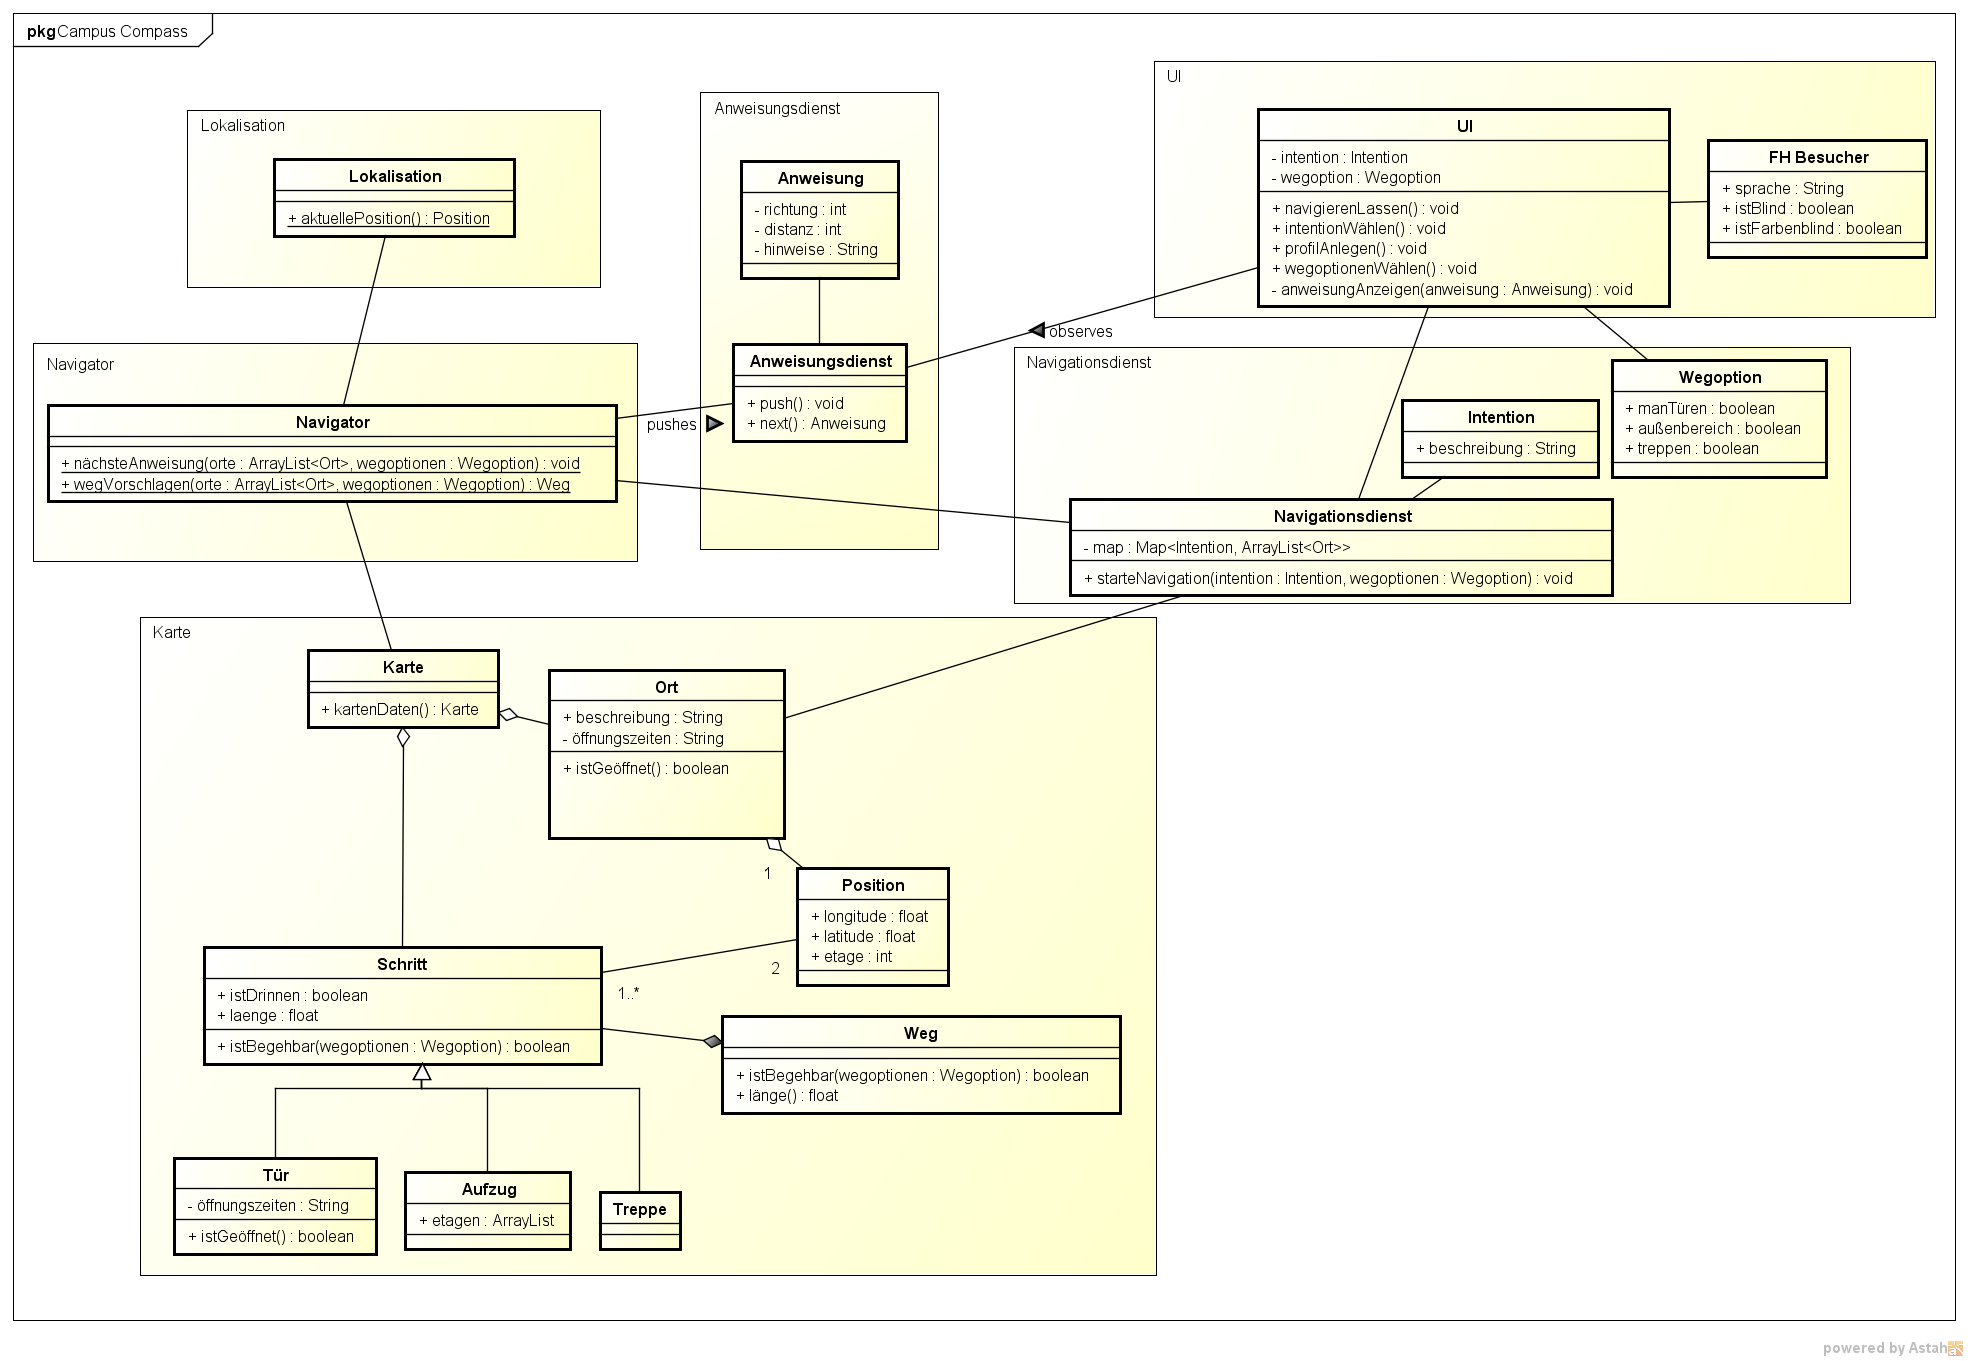
\includegraphics[width=\linewidth]{img/klassendiagramm.png}
  \label{img:klassendiagramm}
  \caption{Klassendiagramm}
\end{figure}

\subsubsection*{Zustandsdiagramm (Verhalten)}
... bieten eine standardisierte Möglichkeit um die zuvor genannten Nutzer und ihre Use Cases sowie die Beziehungen zwischen Use Cases untereinander darzustellen.

\begin{figure}[hbt]
  \centering
  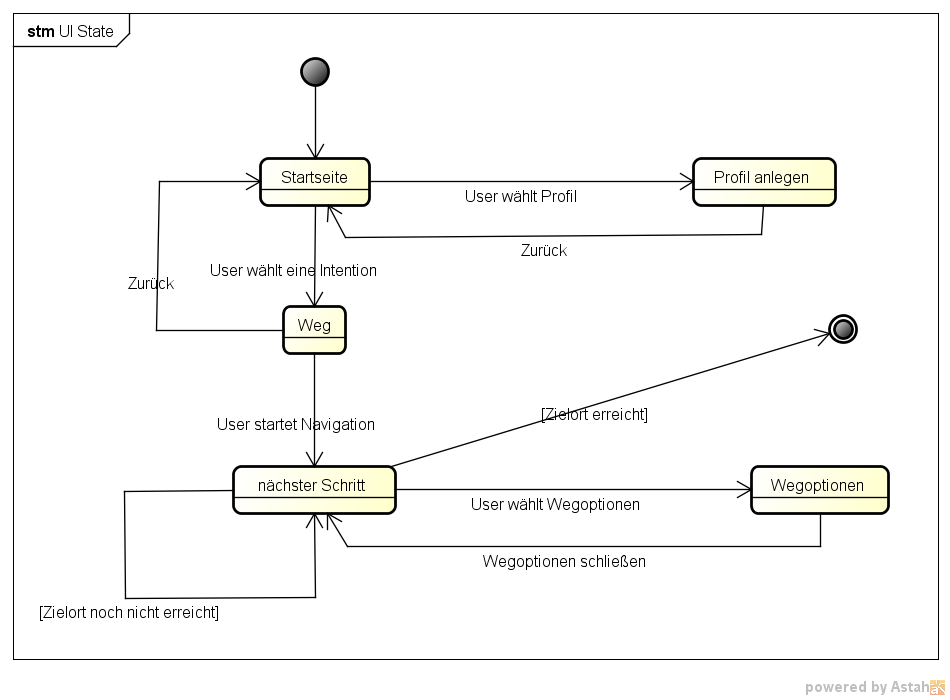
\includegraphics[width=\linewidth]{img/zustandsdiagramm.png}
  \label{img:zustandsdiagramm}
  \caption{Zustandsdiagramm}
\end{figure}

\subsubsection*{Sequenzdiagramm (Verhalten)}
... bieten eine standardisierte Möglichkeit um die zuvor genannten Nutzer und ihre Use Cases sowie die Beziehungen zwischen Use Cases untereinander darzustellen.

\begin{figure}[hbt]
  \centering
  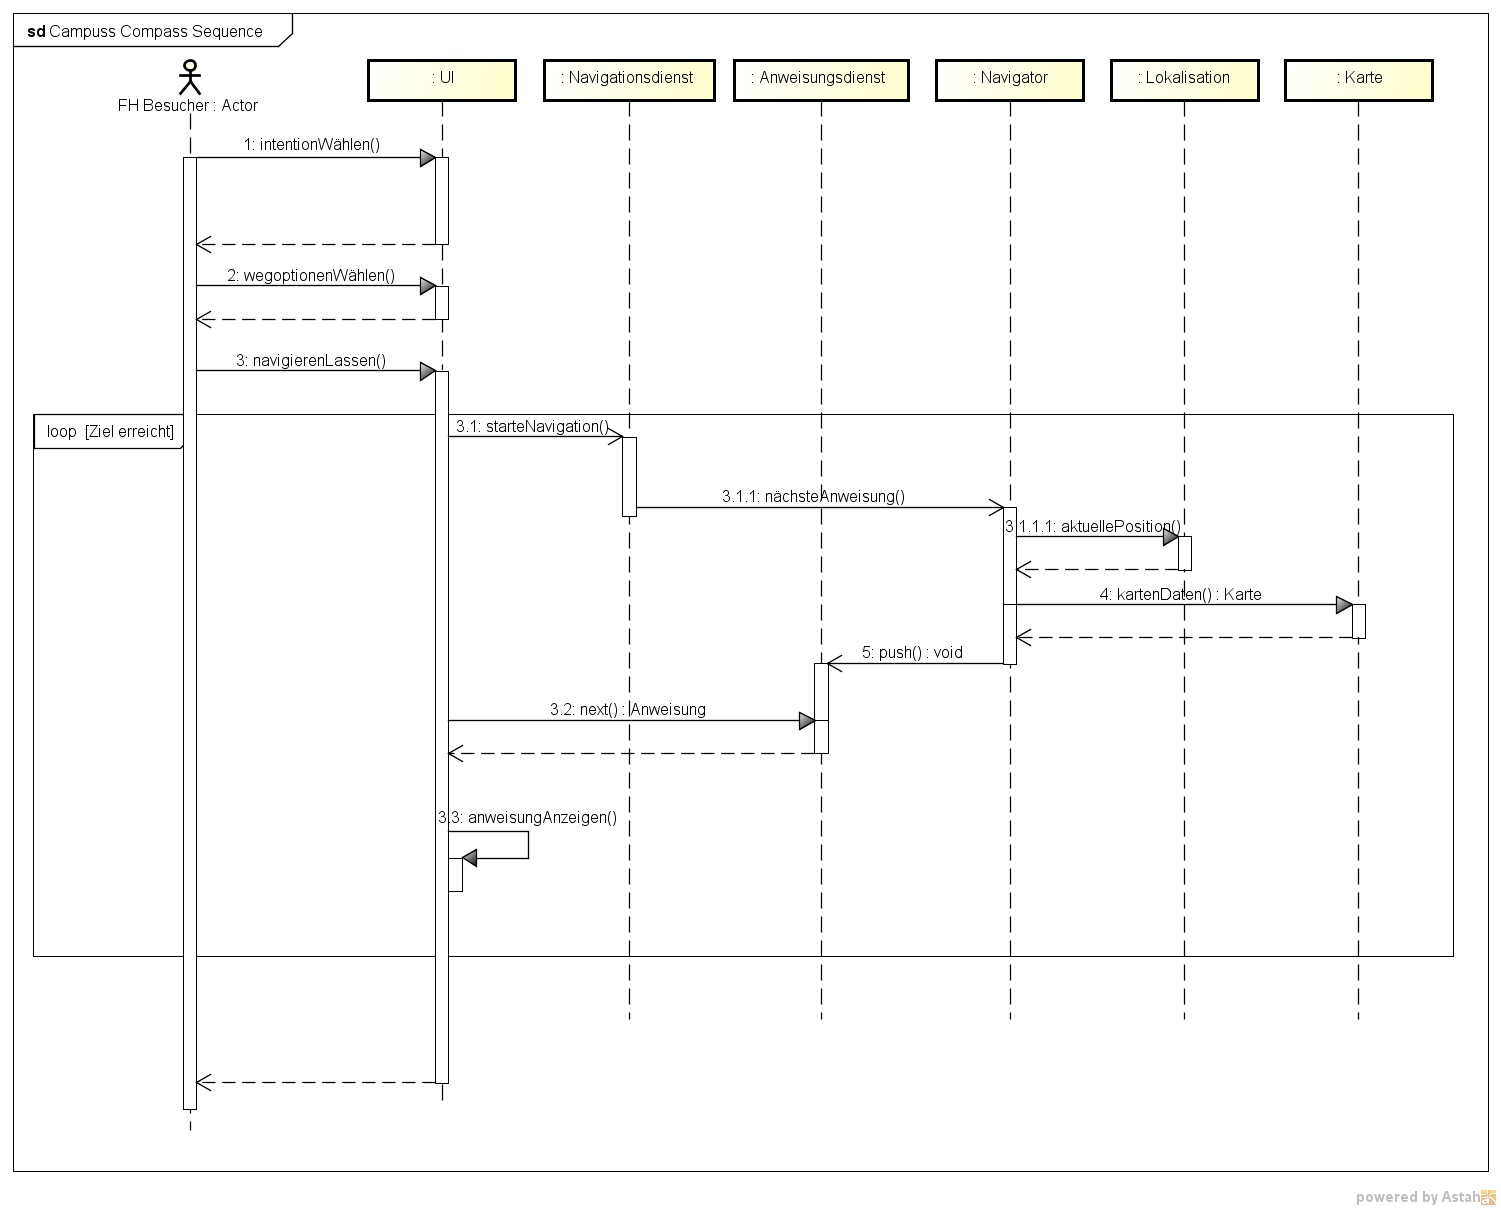
\includegraphics[width=\linewidth]{img/sequenzdiagramm.png}
  \label{img:sequenzdiagramm}
  \caption{Sequenzdiagramm}
\end{figure}